\section{Choice of Auxiliary OOD Dataset in Concept Learning}
\label{app:auxiliary-ood}

Under circumstances where having access to auxiliary OOD dataset for concept learning is not feasible, we suggest that one could use generative methods to generate synthetic dataset, or apply data augmentation techniques. Fig.~\ref{fig:app-augAwA} shows an example of AwA image augmented by \citet{hendrycks2022pixmix}. 

\begin{figure*}[hbt]
\centering
{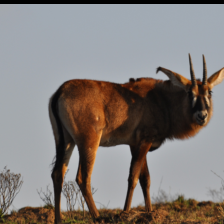
\includegraphics[width=0.2\textwidth]{figures/appendix/9_orig.png}} \hspace{2mm}
{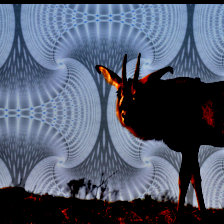
\includegraphics[width=0.2\textwidth]{figures/appendix/9.png}}
\caption{\textbf{Random example of augmented AwA dataset.} 
\textbf{Left:} original image in AwA train set.
\textbf{Right:} corresponding image augmented using the method of \citet{hendrycks2022pixmix}.} 
\label{fig:app-augAwA}
\end{figure*}

We evaluate the effectiveness of our concept learning objective when such augmented AwA train set is used as auxiliary OOD dataset.
Table~\ref{tab:app-auxiliary-ood} illustrates that the generated concepts with augmented AwA (\ie OOD data close to target ID data) have comparable detection completeness and concept separability compared to when MSCOCO (\ie OOD data far from ID data) was used.
But still, further evaluation on generated concept-based explanations with different choice of auxiliary OOD dataset remains as an interesting research question.

\begin{table}[htb]
    \centering
    \begin{adjustbox}{width=1\columnwidth,center}
		\begin{tabular}{l|l|l|c|c|c|c|c|c}
			\toprule
			\multirow{3}{0.001\linewidth}{OOD detector} & \multirow{3}{0.10\linewidth}{Hyper-\\parameters} &
			\multirow{3}{0.05\linewidth}{ $\eta^{}_{\bff}(\bfC) \uparrow$} & \multicolumn{6}{c}{Test OOD dataset} \\ \cline{4-9}
    		& & & \multicolumn{2}{c|}{\texttt{Places}} & \multicolumn{2}{c|}{\texttt{SUN}} & \multicolumn{2}{c}{\texttt{Textures}}\\ \cline{4-9}
    		& & & $\eta^{}_{\bff, S}(\bfC) \uparrow$ & $J_{\textrm{sep}}(\bfC, \bfC') \uparrow$ & $\eta^{}_{\bff, S}(\bfC) \uparrow$ & $J_{\textrm{sep}}(\bfC, \bfC') \uparrow$ & $\eta^{}_{\bff, S}(\bfC) \uparrow$ & $J_{\textrm{sep}}(\bfC, \bfC') \uparrow$ \\ \hline \hline
			%
            % {MSP} & $(10, 0.1, 50)$ & \underline{0.984} $\pm$ 0.0004 & \underline{\textbf{0.960}} $\pm$ 0.0004 & \underline{\textbf{2.756}} $\pm$ 0.0854 & \underline{\textbf{0.961}} $\pm$ 0.0005 & \underline{\textbf{4.442}} $\pm$ 0.0830 & \underline{\textbf{0.937}} $\pm$ 0.0004 & \underline{\textbf{3.587}} $\pm$ 0.2145\\ \hline

            {Energy} 
			& $(1, 0.1, 50)$ & 0.955 $\pm$ 0.0006 & 0.940 $\pm$ 0.0005 & 1.746 $\pm$ 0.0712 & 0.9410 $\pm$ 0.0005 & 3.0703 $\pm$ 0.0580 & 0.927 $\pm$ 0.0005 & 3.417 $\pm$ 0.1419 \\
			\bottomrule
		\end{tabular}
	\end{adjustbox}
        \vspace{2mm}
	\caption[]{Results of concept learning with augmented AwA train set as auxiliary OOD in concept learning.
	}
	\label{tab:app-auxiliary-ood}
\end{table}
